\chapter[Concept Drift]{Concept Drift}
\label{ch:concept-drift}\index{Concept Drift|(}

   Nowadays, huge amounts of data are being generated every day. Such data is providing insights on patterns and its importance is increasing over time, thus making it impossible to collect and process data manually. Moreover, simple data analysis is not sufficient to make educated decisions as the most important knowledge is hidden within the captured data.
   
Classification techniques are within the most utilised algorithms in order to extract hidden patterns. One major limitation of such classification models is the assumption that the underlying data concepts will not change over time. This assumption poses a major classification limitation as in the real-world observations and classes do change over time.  A real-world example is a spam filter where spammers continuously find new ways of how to send spam to increase their success rate.  Thus, a classification technique will decrease it accuracy over time as the observations, statistics and their classifications will not hold forever. This problem is referred to as concept drift. This increases machine learning model's complexity, mostly in those cases where new data is treated as an important contributor to the final concept classification \citep{Bishop:2006:PRM:1162264, Tsymbal04theproblem}. 

Moreover, concept drift refers to the changes within the learned structure which occur over time. These changes could result into mis-classifications and also includes long term and short-term fluctuations may disrupt the underlying classification probability.

\section{Types of concept drift}
In literature one finds five basic types of concept drift which are:

  \begin{figure}[hbt!]
  \centering
      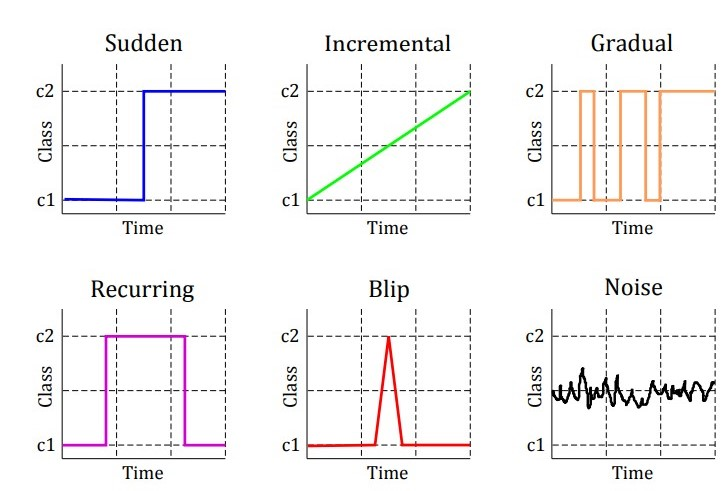
\includegraphics[width=0.88\linewidth]{graphics/concept_drift/concept_drift.jpg}
      \caption{Different types of concept drift excluding noise. \citep{GomezLosada2017}}
      \label{fig:concept-drift-types }
  \end{figure}
  
  
   \begin{enumerate}
  \item Sudden drift: This kind of concept drift, happens in those cases where the concept drift happens abruptly. An example of such drift is season changes in sales \citep{Tsymbal04theproblem}.
  \item Incremental: The drift happens whenever variables change their value over time. An example of this type of drift is the effect of prices due to inflation where prices will keep rising overtime \citep{Tsymbal04theproblem}. 
  \item Gradual drift: Although its similar to incremental, a gradual drift refers to those cases where over time the concept changes definition. Example in a fraud detection, a fraudulent may transition from one category to another and back \citep{Tsymbal04theproblem}.
  \item Recurring drift: This refers to those instances where the classification changes over time and alternates between the classes. A real-world example is the usage of a particular mobile application where a user may use the application differently between work and home \citep{Tsymbal04theproblem}. 
  \item Blip drift: Is an abrupt drift, which only lasts for a very short duration. There has been number of debates over blip if it qualifies as noise or is ignore or the model is adjusted to correctly classify the blip drift. Nonetheless, adjusting the model may harm future classifications as following the blip the old model must be restored. An example of blip drift is Cyber Monday where on-line shops might experience an increase in their sales or page hits which is an abnormal pattern \citep{Tsymbal04theproblem}.
  \item Noise: This refers to insignificant fluctuations which are not connected or related to the target concept. If noise is present, it must be filtered out as it`s not a concept drift and might conflict with the classification model \citep{Tsymbal04theproblem}. 
\end{enumerate}

\section{Detecting Concept drift}

The aim of drift detectors is to raise alarms when concept drift occurs in order to update or rebuild the model. This is a crucial step in models as it increases the robustness and model accuracy.  Two simple drift detectors are the Cumulated Sum (CUSUM) \citep{ROSS2012191} and the Geometric Moving Average (GMA) \citep{ROSS2012191}. The main difference between these detectors is that CUSUM raises an alarm when the sum of the inputted data is not zero whilst GMA considers the weighted average in a window and raised the alarm if the average is higher than a given threshold. 

\section{Dealing with concept drift}
There exist a number of approaches to handle concept drift which mainly are categorized in three approached. Moreover, the aim of these approached is to allow the model to be dynamically updated and adapted to drift without the need of rebuilding which is a costly operation. 
   \begin{enumerate}
  \item Instance selection: Is the most common technique for handling concept drift and its aim is to identify those instances that are truly related to the current concept. This is achieved by creating a form of a moving window which considers recent information whilst utilising learnt prediction concepts in the immediate future. Moreover, due to the fact that the classification will be utilising recent data, the model will be automatically excluding old data \citep{Webb:2016:CCD:2962863.2962874}.

 \item Instance weighting: In this technique instances are weighted depending on their age and relevance to the concept. This allows gradual drift to start being properly handled by the model as new data would have more weight whilst past data would start losing its classification power \citep{Webb:2016:CCD:2962863.2962874}. 

 \item  Ensemble learning: allows one to obtain better classification results by processing the data through multiple algorithms. The resultant of each algorithm is combined and results would be considered in the classification decision. Moreover, one could also introduce weights, which weighting is assigned to the different algorithm based on their classification power and accuracy. One downside of ensemble learning is that the data needs to be processed by every algorithm selected for the model classification \citep{Webb:2016:CCD:2962863.2962874}. 
 
 \end{enumerate}
  
\section{Conclusions}

In this chapter, we introduced and discussed concept drift. Machine learning is increasing its popularity and more real-world application are being released like self-driving cars and fraud detection, which applications do suffer from concept drift. This is due to the fact that data in the real-world is not static, thus concept drift will be residing in such applications and must be dealt with.  
Moreover, one major limitation in concept drift, is the lack of real-data during the experimentation and testing. This is due to the fact that drift data has to be generated artificially, thus, limiting the experiment efficiency. Example, even though Tesla did rigorous testing and were given the go-ahead of releasing self-driving cars, a number of deadly crashed emerged. Thus, concept drift is an important aspect in machine learning as one needs to enable the model to adapt to new concepts or raise alarms if drastic shifts are encountered \citep{Stewart2018}. 